\documentclass[]{article}
\usepackage{lmodern}
\usepackage{amssymb,amsmath}
\usepackage{ifxetex,ifluatex}
\usepackage{fixltx2e} % provides \textsubscript
\ifnum 0\ifxetex 1\fi\ifluatex 1\fi=0 % if pdftex
  \usepackage[T1]{fontenc}
  \usepackage[utf8]{inputenc}
\else % if luatex or xelatex
  \ifxetex
    \usepackage{mathspec}
  \else
    \usepackage{fontspec}
  \fi
  \defaultfontfeatures{Ligatures=TeX,Scale=MatchLowercase}
  \newcommand{\euro}{€}
\fi
% use upquote if available, for straight quotes in verbatim environments
\IfFileExists{upquote.sty}{\usepackage{upquote}}{}
% use microtype if available
\IfFileExists{microtype.sty}{%
\usepackage{microtype}
\UseMicrotypeSet[protrusion]{basicmath} % disable protrusion for tt fonts
}{}
\usepackage[margin=1in]{geometry}
\usepackage{hyperref}
\PassOptionsToPackage{usenames,dvipsnames}{color} % color is loaded by hyperref
\hypersetup{unicode=true,
            pdftitle={When Do Regulators Lean Against the Wind?: The Political Economy of Implementing Macro-prudential Regulatory Tools: Preliminary results},
            pdfauthor={Jeffrey Chwieroth and Christopher Gandrud},
            pdfborder={0 0 0},
            breaklinks=true}
\urlstyle{same}  % don't use monospace font for urls
\usepackage{graphicx,grffile}
\makeatletter
\def\maxwidth{\ifdim\Gin@nat@width>\linewidth\linewidth\else\Gin@nat@width\fi}
\def\maxheight{\ifdim\Gin@nat@height>\textheight\textheight\else\Gin@nat@height\fi}
\makeatother
% Scale images if necessary, so that they will not overflow the page
% margins by default, and it is still possible to overwrite the defaults
% using explicit options in \includegraphics[width, height, ...]{}
\setkeys{Gin}{width=\maxwidth,height=\maxheight,keepaspectratio}
\setlength{\parindent}{0pt}
\setlength{\parskip}{6pt plus 2pt minus 1pt}
\setlength{\emergencystretch}{3em}  % prevent overfull lines
\providecommand{\tightlist}{%
  \setlength{\itemsep}{0pt}\setlength{\parskip}{0pt}}
\setcounter{secnumdepth}{0}

%%% Use protect on footnotes to avoid problems with footnotes in titles
\let\rmarkdownfootnote\footnote%
\def\footnote{\protect\rmarkdownfootnote}

%%% Change title format to be more compact
\usepackage{titling}

% Create subtitle command for use in maketitle
\newcommand{\subtitle}[1]{
  \posttitle{
    \begin{center}\large#1\end{center}
    }
}

\setlength{\droptitle}{-2em}
  \title{When Do Regulators Lean Against the Wind?: The Political Economy of
Implementing Macro-prudential Regulatory Tools: Preliminary results}
  \pretitle{\vspace{\droptitle}\centering\huge}
  \posttitle{\par}
  \author{Jeffrey Chwieroth and Christopher Gandrud}
  \preauthor{\centering\large\emph}
  \postauthor{\par}
  \predate{\centering\large\emph}
  \postdate{\par}
  \date{28 March, 2016}


\usepackage{setspace}\doublespacing
\usepackage{lscape}

% Redefines (sub)paragraphs to behave more like sections
\ifx\paragraph\undefined\else
\let\oldparagraph\paragraph
\renewcommand{\paragraph}[1]{\oldparagraph{#1}\mbox{}}
\fi
\ifx\subparagraph\undefined\else
\let\oldsubparagraph\subparagraph
\renewcommand{\subparagraph}[1]{\oldsubparagraph{#1}\mbox{}}
\fi

\begin{document}
\maketitle

\textbf{Incomplete working draft} containing \textbf{preliminary}
results. Comments welcome.\footnote{Jeffrey Chweiroth is a Professor of
  International Political Economy at the London School of Economics
  (\href{mailto:j.m.chwieroth@lse.ac.uk}{\nolinkurl{j.m.chwieroth@lse.ac.uk}}).
  Christopher Gandrud is a Lecturer of Quantitative International
  Political Economy at City University London and Post-doctoral Fellow
  at the Hertie School of Governance
  (\href{mailto:christopher.gandrud@city.ac.uk}{\nolinkurl{christopher.gandrud@city.ac.uk}}).}

\begin{abstract}
In the aftermath of the global financial crisis, macro-prudential regulatory (MPR) tools, which aim to limit the build-up of systemic risk and the macroeconomic costs of financial instability, have gained widespread attention. An important element of MPR tools involves implementing new counter-cyclical regulatory measures to dampen credit cycles. Yet the political dynamics of MPR tools are potentially complicated in that their implementation involves moving against market and public sentiment during boom periods as well as affecting who can obtain access to financing and who cannot. In this sense, the use of MPR tools can be highly and conspicuously distributional, thus potentially constraining their use and effectiveness. In many cases, the allocation of MPR responsibilities to hitherto independent central banks creates additional concerns about the nature of their accountability relationship with the rest of the political process and the public at large. To shed light on these critical issues, we provide the first cross-national statistical political economy analysis of MPR implementation. Our analysis assesses the relative importance of political credit cycles, institutional demands, and societal demands for credit tightening and easing.
\end{abstract}

\clearpage

\section{Introduction}\label{introduction}

In the wake of the global financial crisis, politicians, regulators, and
central bankers have turned to a new macro-prudential regulatory
philosophy aimed at limiting the build-up of systemic risk and the
macroeconomic costs of financial instability. As opposed to the
pre-crisis micro-prudential focus on protecting the integrity of
individual financial institutions, markets, and instruments, an
important element of this philosophy prioritizes the creation of new
counter-cyclical regulatory tools. Much faith is now being placed in the
efficacy of these tools in preventing and mitigating the costs of the
next financial crisis. Some of this faith is based on the perceived
success of macro-prudential regulation in places such as East Asia and
Canada.

However, we presently lack a coherent understanding of the
context-specific political constraints that may shape what
macro-prudential tools are actually used and how. These constraints may
dramatically limit what tools are feasible in a given context and could
lead to unintended negative consequences. For example, as part of the
shift to a focus on macro-prudential and counter-cyclical regulation,
central banks in a number of places, such as the United States, United
Kingdom, and the Eurozone, have been given greater regulatory authority.
These central banks have previously been very successful in fighting
inflation. However, it is uncertain if this success will transfer over
to the newly created macro-prudential regulations. Macro-prudential
regulation could be a much more politicised issue than monetary policy
in these contexts. Regulators may be biased either towards
non-intervention, because they would be subject to political pressure
against tightening during a boom, or towards intervention, because they
would face less criticism for puncturing a non-bubble than for failing
to spot a real one. Perceived regulatory failures could end up eroding
the reputations of central banks, thus damaging their ability to curtail
inflation.

The existing literature says little about the salient political features
that shape how regulators respond to these pressures. We thus clearly
need a better understanding of how the political economy context shapes
regulatory systems.

\section{Economic Conditions and Macro-prudential Policy
Choices}\label{economic-conditions-and-macro-prudential-policy-choices}

{[}JEFF FILL IN{]}

\section{Political Conditions and
Macro-prudential}\label{political-conditions-and-macro-prudential}

{[}JEFF FILL IN{]}

\section{Dependent variables}\label{dependent-variables}

Our two dependent variables are derived from a new data set of
macro-prudential regulatory (MPR) actions created by Reinhardt and
Sowerbutts (2015). Aggregating a number of sources, mostly from IMF
staff economists, and supplemented with additional hand-coded incidents,
they generated binary quarterly indicators of MPR tightening and
loosening for 70 countries between 1990 and 2014. They created dummies
for a range of individual MPR instruments including lending standards,
reserve requirements, capital regulation, risk weights, underwriting
standards, profit distribution, and loan to value ratios.

Given that in the sample the use of some of these policies is rarely
observed, we created two summary dummy variables from the Reinhardt and
Sowerbutts (2015) data to use as our dependent variables. One variable
captured if a country took an action that Reinhardt and Sowerbutts
(2015) classified as MPR tightening in a given quarter. The other
dependent variable captures loosening. These variables equal one for
each country-year that any macro-prudential policy was tightened or
loosened, respectively, and zero otherwise. Figure \ref{describe_cumsum}
shows the cumulative sum (from the year 2000) of these policies for each
country-year in our sample.

\section{Right-hand variables}\label{right-hand-variables}

We examined how a number of political and economic factors may affect
decisions to tighten and loosen macro-prudential policy.

Governments may feel a need to tighten macro-prudential policy when
asset prices are rising. A key asset price, often discussed regarding
macro-prudential policy, are \textbf{residential property prices}. We
focus on the change in property prices as differences in the level can
be caused by complex sets of idiosyncratic long-term factors which
policy-makers likely do not focus on. Measuring national-level
residential property prices is notoriously difficult (see Scatigna,
Szemere, and Tsatsaronis 2014). We use the 57 national series selected
by the Bank of International Settlements (BIS, Bank of International
Settlements 2016) to be as comparable as possible. The indices are at
quarterly intervals and in terms of real year-on-year percentage change.

Similarly, governments would be more likely to tighten when there are
credit bubbles in order to head off unsustainable lending that could
lead to a crisis. To test for this we gathered data from the (BIS) on
quarterly \textbf{credit provided to the non-financial sector} as a
percentage of GDP. As with housing prices, we focus on changes to credit
provision as levels of credit provision can vary between countries for
many long-term idiosyncratic factors that do not indicate a bubble. We
used this data to create a variable of year-on-year change in credit.

As macro-prudential policy is broadly an attempt to strengthen financial
markets, it is important to include the financial market stress
policy-makers perceived in real-time. To do this we use the
\textbf{FinStress} measure from Gandrud and Hallerberg (2015). They
created a real-time indicator of financial market stress for over 180
countries between 2003 and 2011 using a text analysis of \emph{Economist
Intelligence Unit} monthly country reports. The value ranges from zero
(low stress) to one (high stress). We converted this monthly variable to
country-quarter averages. We do not include FinStress in all of the
models below because it shrinks the time periods of our sample.

We examined a number of other economic indicators from the World Bank's
Development Indicators (World Bank 2016).\footnote{The indicator IDs are
  NY.GDP.MKTP.KD.ZG, FS.AST.DOMS.GD.ZS, and FP.CPI.TOTL.ZG,
  respectively. Note that we created the domestic credit growth variable
  by finding the year-on-year percentage change in domestic credit as a
  percentage of GDP.} These included the \textbf{GDP growth} and
\textbf{domestic credit growth}. GDP growth is our focus.
Macro-prudential policy may be used to calm asset price bubbles, as such
we would expect more tightening when growth is high. We may expect that
governments would loosen MPR when growth and specifically domestic
credit growth is low in order to stimulate the economy. Unfortunately
domestic credit growth data is not widely available and so we have a
limited ability to directly examine this mechanism. Additionally, from
the World Bank Development Indicators, we include \textbf{inflation
rate} as a control. All World Bank Development Indicators are recorded
at the annual level.\footnote{We also examined models with one year lags
  of these variables. In general these lags were not statistically
  significant.}

Policy-makers may turn to macro-prudential tools when they lack the
monetary policy tools needed to constrain bubbles. To test this we
included countries annual average standardised \textbf{central bank
policy interest rate}. This data is from the IMF's International
Financial Statistics (International Monetary Funds 2016). Perhaps
countries with already high policy rates--and thus little room to
maneuver are more likely to turn to MPR policy tools. We also used this
variable to create a measure of central bank policy interest rate
year-on-year percentage change to examine if the rate of change, not
just the level may be important. Macro-prudential and monetary policies
may be treated as complementary--countries could tighten monetary policy
and macro-prudential policy simultaneously to avoid or quell
bubbles--or, conversely, the policies they may be treated as
substitutes. This is an empirical question that we examine below.

We also examined whether or not a countries' \textbf{exchange rate
regime} impacted their propensity to use macro-prudential tools. Perhaps
having a more fixed exchange rate regime would prevent policy-makers
from using monetary policy to tame credit cycles. To examine this we
used the Ethan Ilzetzki and Rogoff (2010) coarse measure of exchange
rate regime. Their measure had six categories, where higher values
indicated more a flexible exchange rate regime. It is available through
2010. However, we did not find any meaningful results with this measure
and do not include it among the estimates below.

Elected politicians may find it difficult to tighten macro-prudential
policy generally as this may slow economic growth in the short-term,
even if it promotes stability in the future. Countries with more
\textbf{central bank independence} (CBI) suffer less from such a time
inconsistency problem. Independent central banks were created under the
rational that they would not suffer from the electorally induced
time-inconsistency problems in monetary policy-making faced by elected
politicians. So, countries with independent central banks may be more
likely to tighten MPR. We use a standard measure of CBI first devised by
Cukierman, Web, and Neyapti (1992) and recently updated through 2008 for
about 80 countries by Bodea and Hicks (2015). It ranges from 0.120 to
0.95 in the sample with higher values indicating more central bank
independence. All countries in the Eurozone have the same CBI score. The
data in Bodea and Hicks (2015) extends to 2010. We assume that CBI was
constant through 2011.

Central bank independence should have a more important role on
tightening if the central bank plays a larger part in macro-prudential
decision-making. To examine this, we included the central bank' and
ministry of finance's--who are presumably more attuned to voters and
removal pressures--de facto involvement in the macro prudential
decision-making. This data was from Lim et al. (2013). Their
\textbf{MaPP} (measuring central bank involvement) and \textbf{MoF}
indices range from a low of zero where there is no involvement to 4
where these actors are primarily or solely responsible. Note that
surprisingly, these measures were never statistically meaningful in our
various estimation models and results with them are not shown below.

It may be that politicians that are more accountable to voters with
short-time horizons and who benefit from easy credit would be less
likely to tighten monetary policy. To examine this possibility, we used
\textbf{Unified Democracy Scores} (UDS) from Pemstein, Meserve, and
Melton (2010) which they updated through 2012. UDS scores are found
using a Bayesian latent variable model of eleven commonly used measures
of democracy. We used the posterior mean estimates from this model. The
variable ranges from about -2.1 to 2.2 where higher scores indicate a
higher level of democracy.

One possible manifestation of electoral accountability effect may be a
macro-prudential regulatory policy electoral cycle. Elected politicians
may be more likely to loosen and less likely to tighten macro-prudential
policy if they are close to an \textbf{election}. Doing so would spur
(slow) credit provision to the economy that voters would like (dislike).
To examine this we gathered executive election dates from Hyde and
Marinov (2012).\footnote{We used Version 4 of the data set.} Politicians
would likely not only loosen or avoid tightening in the immediate
election quarter, but also in the quarters leading up to the election.
As such, we created a binary executive election variable that was one in
the election quarter and the three previous quarters. It was zero
otherwise.

Perhaps politicians' \textbf{economic ideology} may play a role in
macro-prudential decisions. To test this we include the government
executive's economic policy orientation from the Database of Political
Institutions (DPI, Beck et al. 2001 updated through 2012), It is one for
right-leaning, two for centre-leaning, and three for left-leaning. We
never found any support for this variable, so results from models using
it are not shown below.

\textbf{Inequality} may also influence the implementation of
macro-prudential policy measures. Rajan (2012) and Calomiris and Haber
(2014) suggest inequality may be a root cause of credit booms in
democracies, especially in societies with limited redistributive
capacity or political will. Faced with such conditions, democratic
governments may aim to boost the consumption of lower-income households
by manufacturing credit booms through less stringent financial
regulation. Indeed, Piketty and Saez (2013) show that large increases in
private debt before the Great Depression and Great Recession were
associated with widening income inequality. Politicians may prefer not
to intervene and instead permit credit bubbles to inflate in order to
sustain their popularity. To assess the influence of inequality, we use
several standard measures of the Gini coefficient, devised by Solt
(2008) and later updated in Solt (2014). The measures range from zero to
one, with higher values indicating higher income inequality. The first
two measures--market-income Gini and net-income Gini--capture the income
distribution before and after public redistributive measures are taken
into account, respectively. If inequality is an important component of
the MPR decision-making process then we would expect that the inequality
measure that takes redistribution would be more strongly associated with
a low probability of macro-prudential tightening as it would reflect the
public's lived level of inequality.

We use these measures to also assess the extent of public
\textbf{redistribution} on MPR decisions. To do this we created a
measure of redistribution relative to market inequality (the difference
between the market-income and net-income Gini indices divided by
market-income and multiplied by 100); that is, the percentage by which
market-income inequality is reduced by redistribution. Perhaps countries
that respond to inequality pressures with redistributive policies would
be less likely to forestal MPR tightening.

\begin{landscape}
\begin{figure}
    \caption{Cumulative Decisions to Loosen and Tighten Macro-prudential Regulatory Policy (from 2000)}
    \label{describe_cumsum}
    \begin{center}
        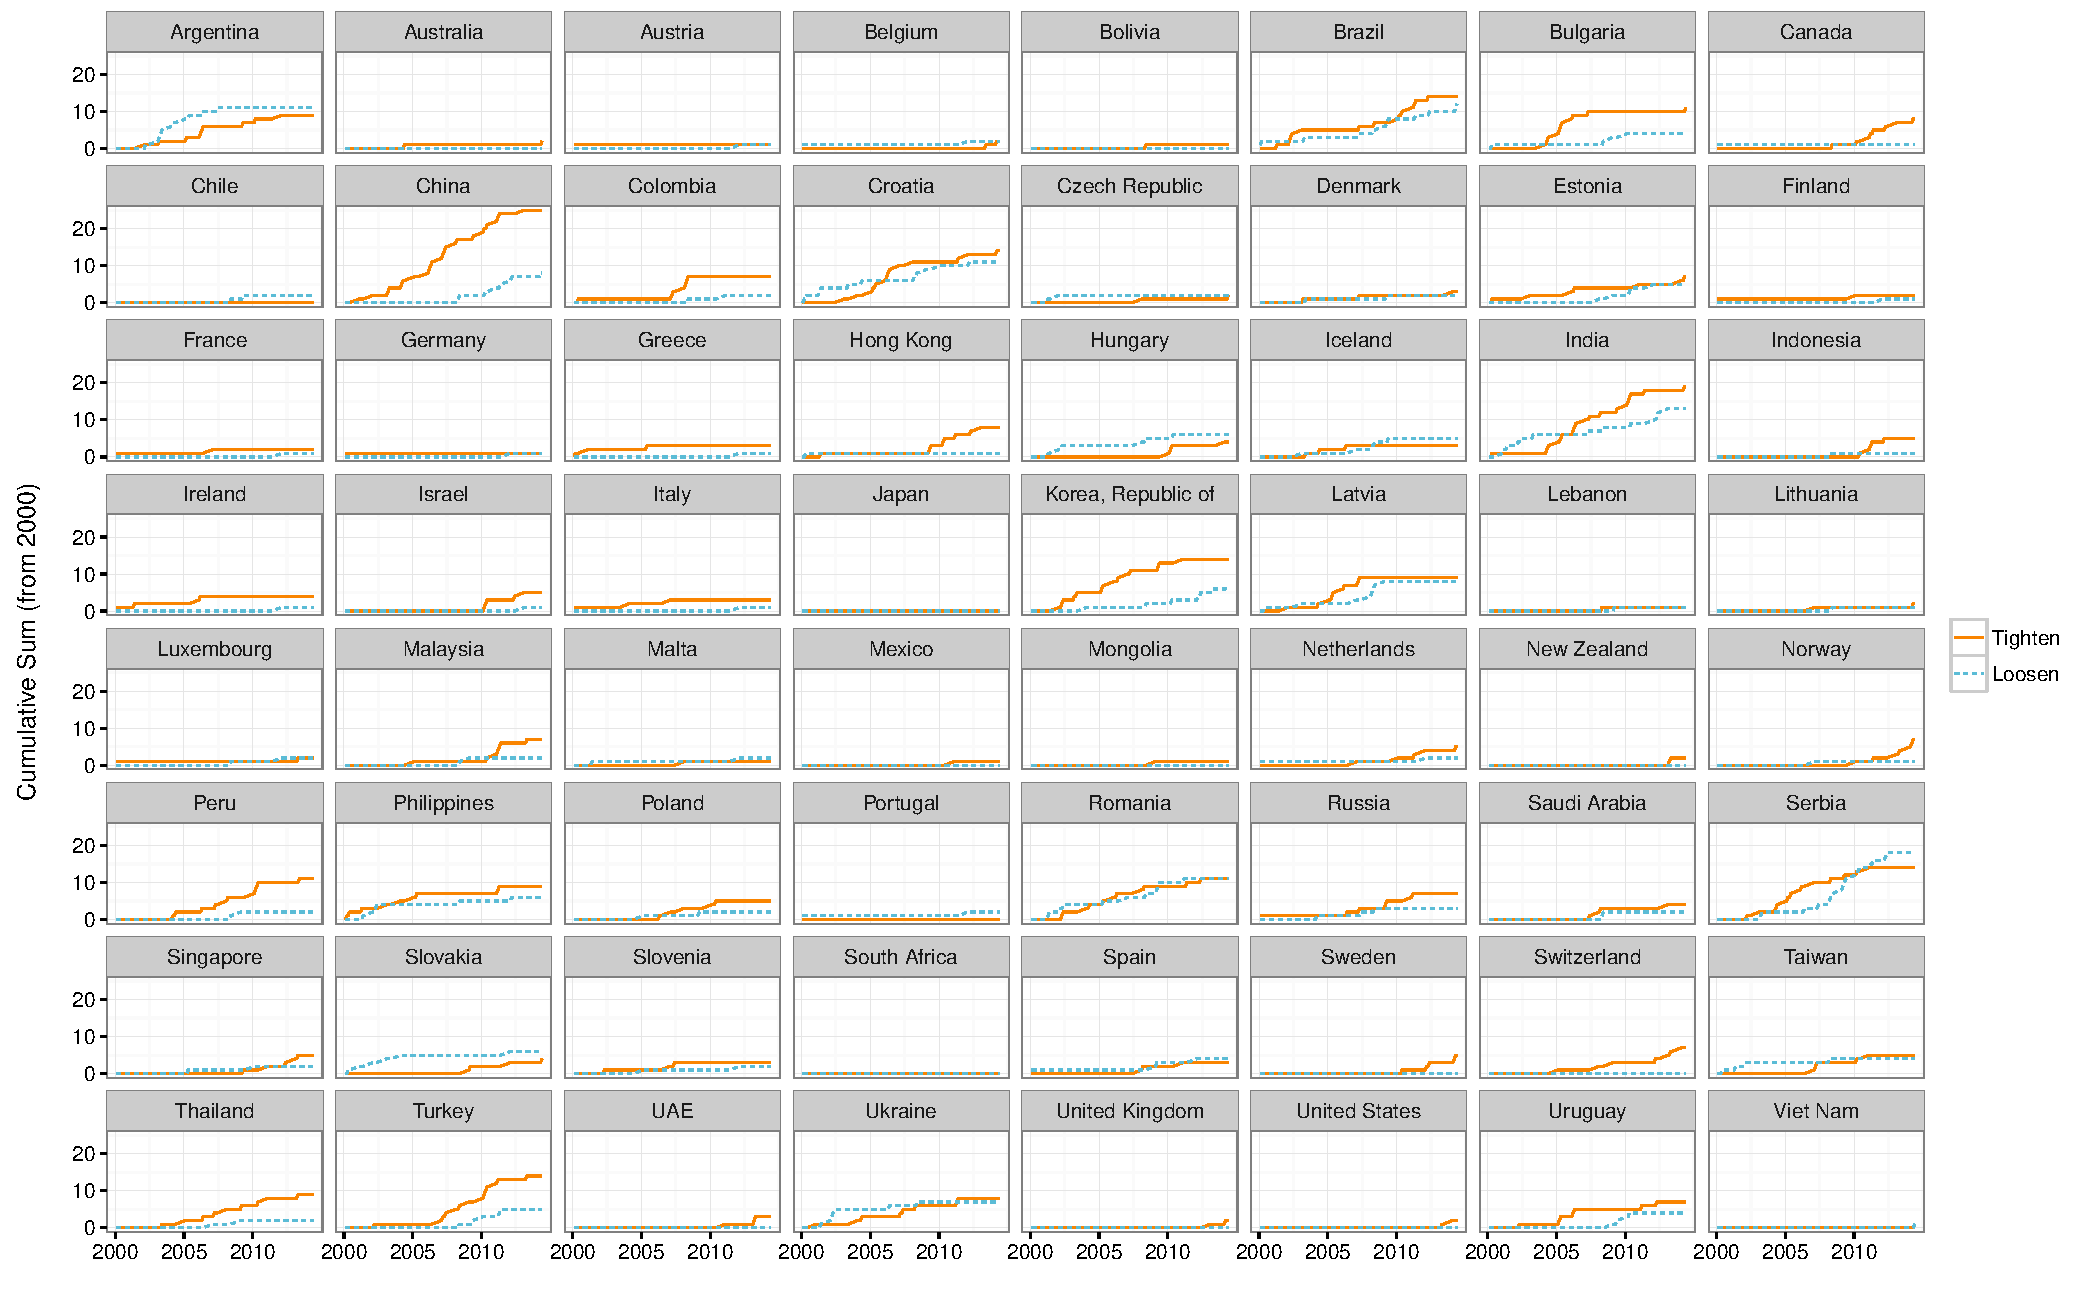
\includegraphics{figures/cumsum_mpr.pdf}
    \end{center}

\end{figure}
\end{landscape}

\section{Preliminary results}\label{preliminary-results}

One possible estimation method for examining our binary dependent
variables would be logistic regression. However, our data does not fit
nicely into this modeling technique. Many of right-hand variables are
strongly correlated with one another, presenting issues of
multicolinearity (see the Online Appendix for the correlation matrix of
our key independent variables) and likely violate the assumptions of the
logistic and similar regression models. There are also relatively few
events to non-events.\footnote{In the full sample there were 5118
  country-quarters, 355 observations country-quarters with any MPR
  policy tightening and 205 instances of loosening. A common way of
  addressing this type of situation is to use rare events logistic
  regression (King and Zeng 2001). Muchlinski et al. (2016) show that
  random forests outperform these types of models in prediction. See
  also the Online Appendix for the event counts in the modeling sample.}
We also have many predictors when including fixed effects relative to
the number of observed monetary policy decisions. All of these issues
point to the usefulness of an alternative modeling strategy: random
forest classification (Breiman 1996; Breiman 2001).

A random forest is a non-parametric method that allows us to include
many correlated variables in the same estimation model (Jones and Linder
2015). Though previously rarely used, this method is increasingly relied
on in political science (e.g. Gandrud and Hallerberg 2015; Hill and
Jones 2014; Jones and Linder 2015; Muchlinski et al. 2016; Shellman,
Levey, and Young 2013; Spirling 2012). The algorithm builds on a method
know as Classification and Regression Trees (CART). A CART algorithm
starts with the complete data set (root node) and recursively partitions
(branches) the observations into increasingly homogeneous groups on the
predictor space based on their values of the predictor variables (see
Muchlinski et al. 2016, 92). This creates a single classification tree.
However, CART creates problems of overfitted trees. Random forests help
overcome this problem by finding multiple trees for bootstrapped samples
of the data and then averaging over the trees. This method allows us to
explore our data set of relatively rare events and find potential
non-linearities and interactions among our correlated variables, which
would be difficult in a logistic regression context. It also has high
robustness to noise and outliers (Muchlinski et al. 2016, 93), which as
we will see, of which there are important instances in the data.

We also ran confirmatory analyses using logistic regression models with
stepwise included right-hand variables and minimally informative prior
information (Gelman et al. 2008) to avoid creating unreasonably large
coefficient estimates. The results of these models will presented in the
Online Appendix.

\subsection{Random Forests: MPR
Tightening}\label{random-forests-mpr-tightening}

We first examined random forests with macro-prudential regulatory policy
tightening as the response variable. To assess each variable's relative
performance for classifying country-quarters as experiencing MPR
tightening or not we first examined the variables' permutation
importance. Permutation importance (Breiman 2001) is found by noting the
prediction error on the out-of-bag (OOB) data. For a given variable, OOB
cases are then randomly permuted in the variable and the prediction
error is recorded. The variable importance for the given variable is
found by averaging the difference between the permuted and unperturbed
error rates. Variable importance for the MPR tightening model are show
in Figure \ref{imp_tighten}.

\begin{figure}
    \caption{Variable Permutation Importance for Classifying Macro-prudential Policy Tightening}
    \label{imp_tighten}
    \begin{center}
        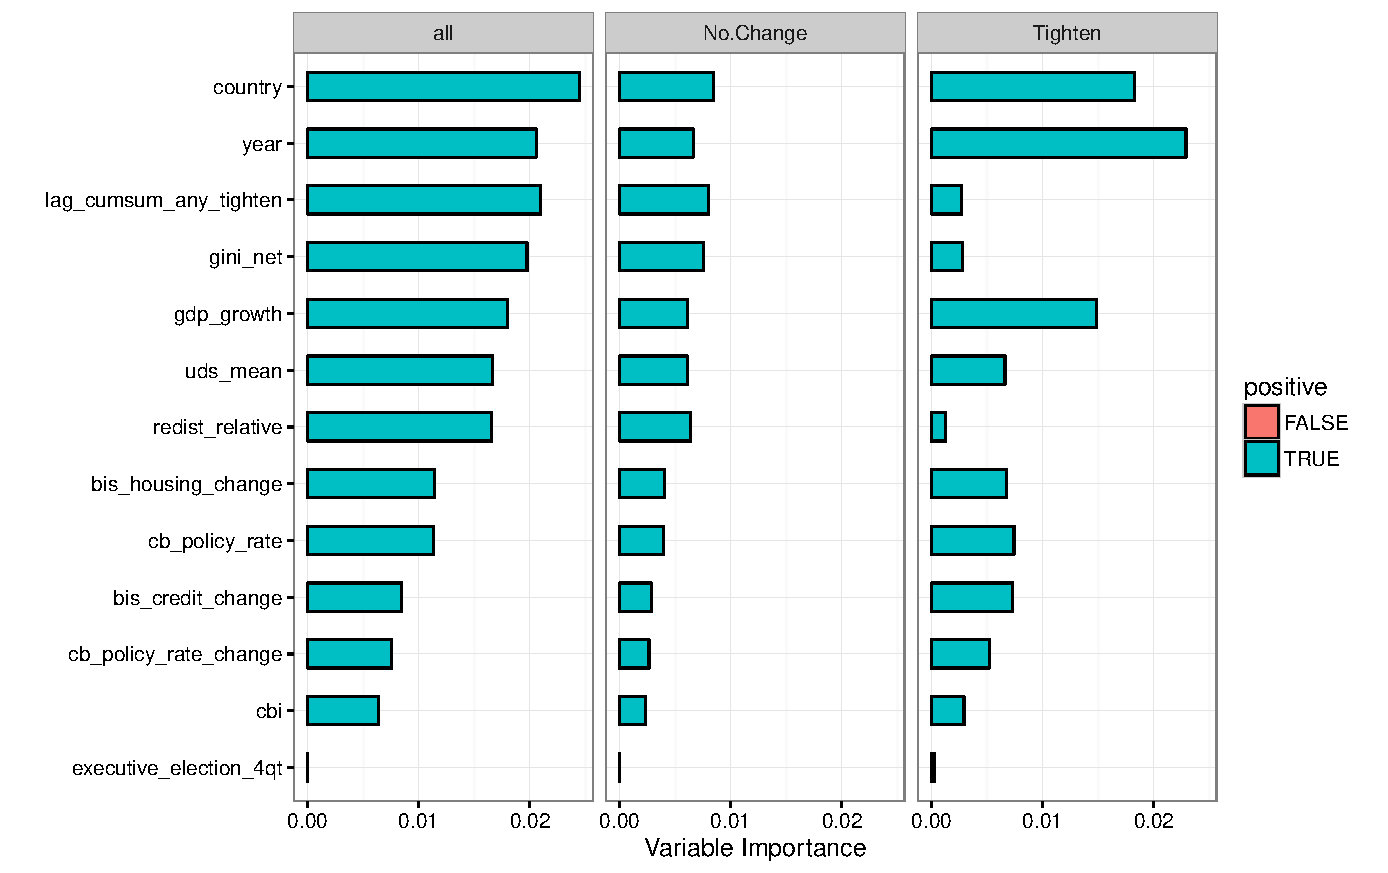
\includegraphics{figures/tighten_imp.pdf}
    \end{center}

    {\scriptsize{Bars coloured by negative or positive variable importance.}}

\end{figure}

The country and year ``fixed effects'' have high variable importance,
especially for decisions to tighten MPR. This suggests that there are
likely other important unobserved factors that vary by country and time
contributing to MPR policy tightening decisions. As we will see below
when looking at partial dependences (see Figure \ref{partial_tighten}),
the year variable is clearly capturing features of the Global Financial
Crisis not picked up by the economic variables. GDP growth is also
relatively important. Conversely, elections, inequality, redistribution,
and central bank independence are found to be relatively unimportant.
Note that we also examined another measure of variable
importance--minimum depth. Results are shown in the Online Appendix.

To get a sense of the estimated form of the variables' effects, we found
their partial dependences with MPR tightening. These are shown in Figure
\ref{partial_tighten}. Partial dependence is calculated by finding the
average prediction from the random forest for each value of \(X = x\)
variable of interest over all other covariates in \(X\) using:\footnote{Largely
  for computational reasons, for variables with many values predictions
  are made for a subset of the values.}

\begin{equation}
    f(x) = \frac{1}{n}\sum_{i=1}^{n}f(x,\; x_{i,o}).
\end{equation}

\(f\) is the predicted MPR policy tightening decision. \(x\) is the
variable for which we want to find the partial dependence and
\(x_{i,o}\) are the other variables (see Friedman 2000; Ehrlinger 2015b,
16). Given the binary dependent data the summand is the log of the
fraction of total votes for the classification--the predicted logit--of
\(y\) defined by:

\begin{equation}
    f(x) = \mathrm{log}p_{k}(x) - \frac{1}{K}\sum_{j=1}^{K}\mathrm{log}p_{j}(x).
\end{equation}

\(K\) is the number of classes in \(y\). \(k\) is the predicted class.
\(p_{j}\) is the proportion of votes for class \(j\) (Muchlinski et al.
2016, 99). We can think of partial dependence as the average predicted
probability of MPR tightening for a value of one explanatory variable
averaged within the joint values of the other predictors (Jones and
Linder 2015, 8) or possibly in more familiar terms: the marginal effect
of a variable on the probability of tightening (Muchlinski et al. 2016,
98).

\begin{figure}
    \caption{Partial Dependence Plot for Macro-prudential Regulatory Policy Tightening}
    \label{partial_tighten}
    \begin{center}
        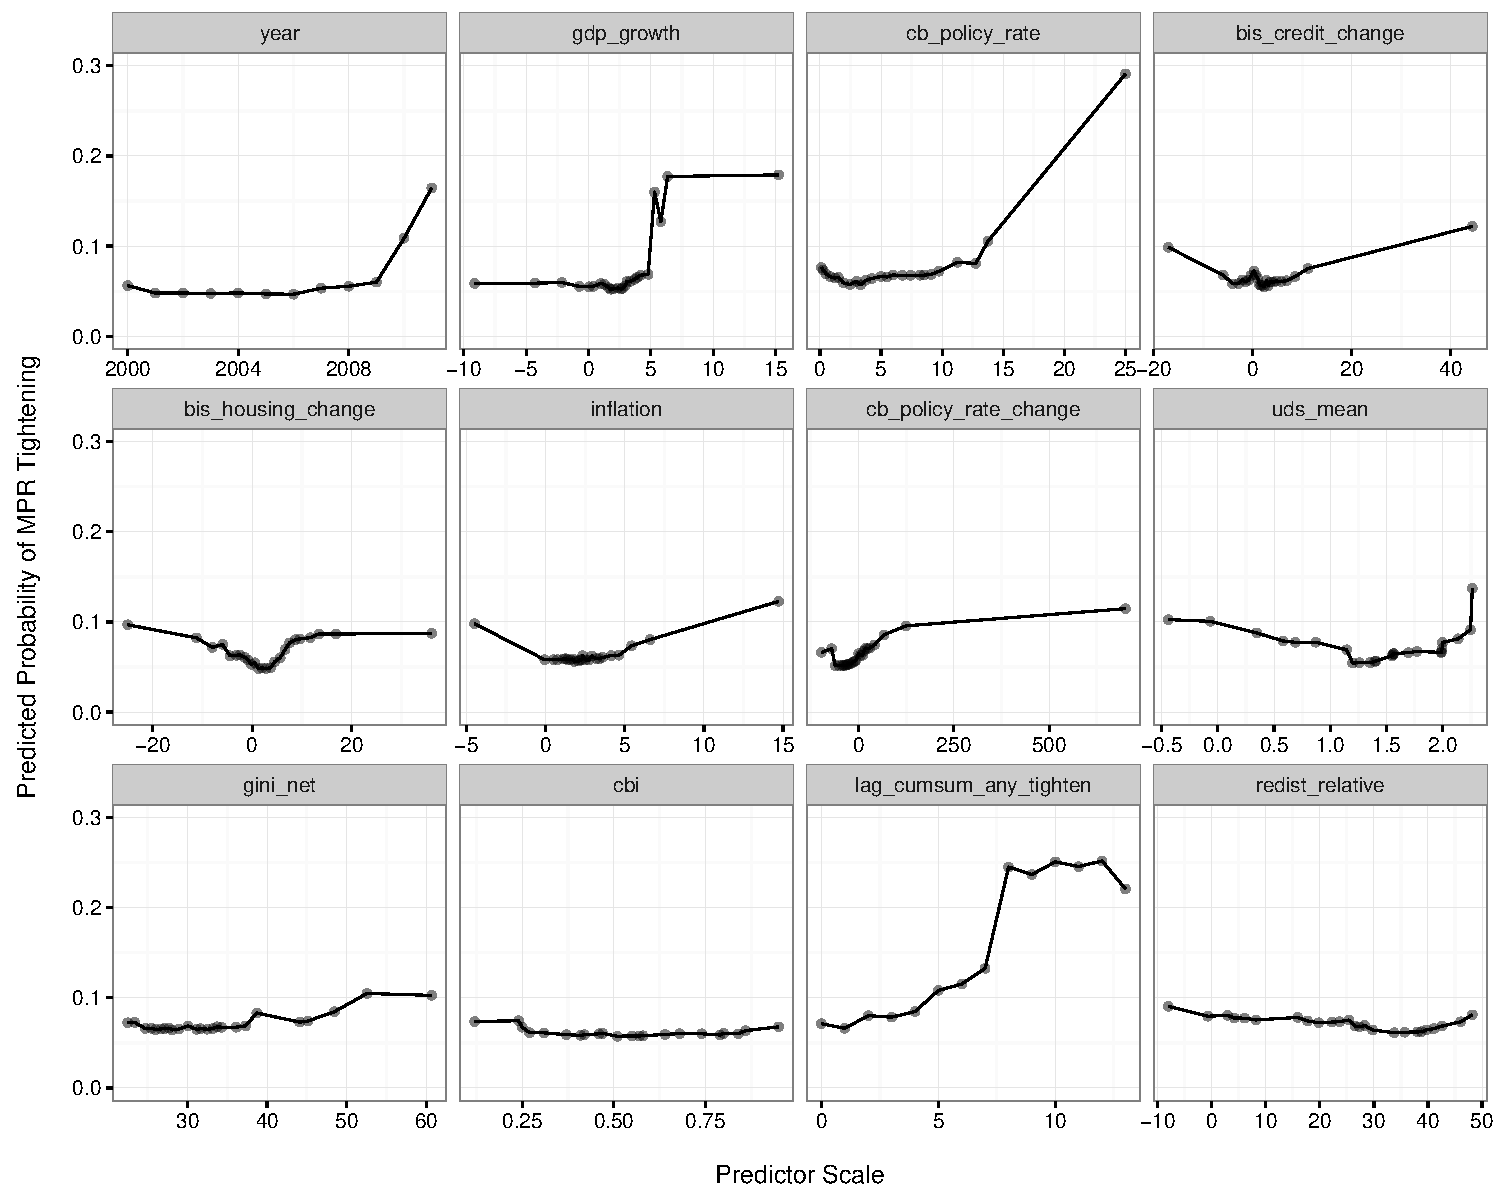
\includegraphics{figures/patial_tighten.pdf}
    \end{center}

    {\scriptsize{Variables shown are those that have non-negative variable importance. The "fixed effect" variables country variable is also not shown. Note that predictions are for policy change to be made per quarter.}}

\end{figure}

Countries with higher central bank policy rates have a higher
probability of tightening. There does not appear to be much difference
in the low probability of tightening if the policy rate is below about
10 percent. Above this point the predicted probability of tightening
increases to between 10 to about 30 percent. This result appears to be
largely driven by Brazil which tightened in nine quarters between 2002
and 2010. Brazil was only one of four countries to have such a high
policy rate in the estimation sample. One of the other
countries--Columbia in 2000 also tightened.\footnote{The other two
  countries were Indonesia and South Africa.} As such it appears that
countries with less monetary policy room for maneuver, are more likely
to resort to macro-prudential tightening. Interestingly, countries with
increasing policy rates are also more likely to tighten. This suggests
that macro-prudential tightening may be used as a complement to monetary
policy tightening.

GDP growth appears to have a relationship with MPR tightening in a
manner that we would expect from a model of policy-makers tightening in
an attempt to calm bubbles. There is a very low probability of MPR
policy tightening at growth levels up to about 5 percent of GDP. From
this point, the probability of tightening rises somewhat, reaching
almost 20 percent per quarter.

Housing price changes appear to have a U-shaped relationship with MPR
tightening. When housing prices are stable--around zero percent
change--there is around a 5 percent probability of tightening. Large
year-on-year quarterly housing price increases almost double the
probability of tightening to a little under 10 percent per quarter. This
is what we would expect from policy-makers using MPR policy tightening
to quell property price bubbles. Interestingly, large housing price
declines are also associated with tightening. The countries in the model
where housing prices declined more than 5 percent and had tightening
include Brazil, Canada, Singapore, and Spain. Brazil tightened reserve
requirements. The others tightened lending standards following the start
of the Global Financial Crisis, despite falling housing prices. Given
the wider crisis context in which these countries tightened, it may be
that their policy moves were intended to prevent banking system
contagion from an external crisis that was already hitting economic
growth and so housing prices. We see a possibly similar Global Financial
Crisis effect by looking at the partial dependence for the year
variable. The predicted probability of tightening increases noticeably
from 2009. We that changes in credit provision to non-financial
institutions has a broadly similar, though shallower partial dependence.

Having already instituted a MPR measure greatly increases the
probability of doing it even. We can see this by looking at the partial
dependence for the cumulative sum of previous policy tightening
measures. To a certain extent this finding likely reflects unobserved
factors that incline a country to tighten. At the same time, it could
also indicate that once countries begin to put MPR tools in their policy
toolbox, that they are more likely to rely on them in the future.

We never found any reasonable evidence that elections play an important
role in predicting MPR tightening (see the Online Appendix for further
details). This suggests against the idea of a macro-prudential electoral
cycle. Additionally central bank independence is almost not an important
predictor using various importance measures and by looking at its
partial dependence. These two findings complement each other. If there
is not a macro-prudential electoral cycle, then countries with and
without independent central banks would not have meaningful differences
in tightening choices as the purported effect of CBI would be to
mitigate MPR electoral cycles.

While we may not have found evidence that electoral cycles influence MPR
tightening decisions, democratic accountability in general does seem to
have some relationship. Less democratic countries, measured by having
lower UDS scores are more likely to tighten than those with higher
scores, suggesting that politicians in less democratic countries are
under less pressure to maintain credit levels to please voters. There
are notable exceptions, however. The very democratic countries of
Canada, Finland, Norway, Sweden, and Switzerland all tightened in the
sample.

There is some weak evidence that inequality and redistribution change
the probability of tightening, though not in the way we initially
expected. Based on the previous literature, we anticipated that
countries with higher inequality, especially even after redistribution,
would be less likely to tighten in order to not alienate less advantaged
supporters by reducing their access to credit. However, we found that
countries with higher inequality (using both the market and
post-redistribution measures, though only the latter is included in the
model shown) are more likely to tighten. Similarly, countries with less
redistribution are slightly more likely to tighten. Countries such as
Brazil, Colombia, Peru, and Thailand all had Gini scores above 45 (on
both measures) and tightened over multiple quarters. Almost all of these
countries tightened by increasing reserve requirements. One possible
explanation for these results that seem to contradict expectations is
that while there may be political pressures to not tighten in unequal
societies, they are also more likely to get into situations where they
need to tighten. These countries also seem to tighten in such a
away--increasing reserve requirements--that does not immediately impact
borrowers, though presumably such policies would tighten available
credit over the medium-term.

\subsection{Random Forests: MPR
Loosening}\label{random-forests-mpr-loosening}

It is important to note a few data caveats about macro-prudential
loosening. Chiefly, many instances of MPR loosening occurred in the most
recent period of our sample as countries began to wind down their
responses to the Global Financial Crisis. However, we lack data on many
of our covariates after 2011. As such, our effective sample of MPR
loosening decisions is very limited.

\begin{figure}
    \caption{Variable Permutation Importance for Classifying Macro-prudential Policy Loosening}
    \label{imp_tighten}
    \begin{center}
        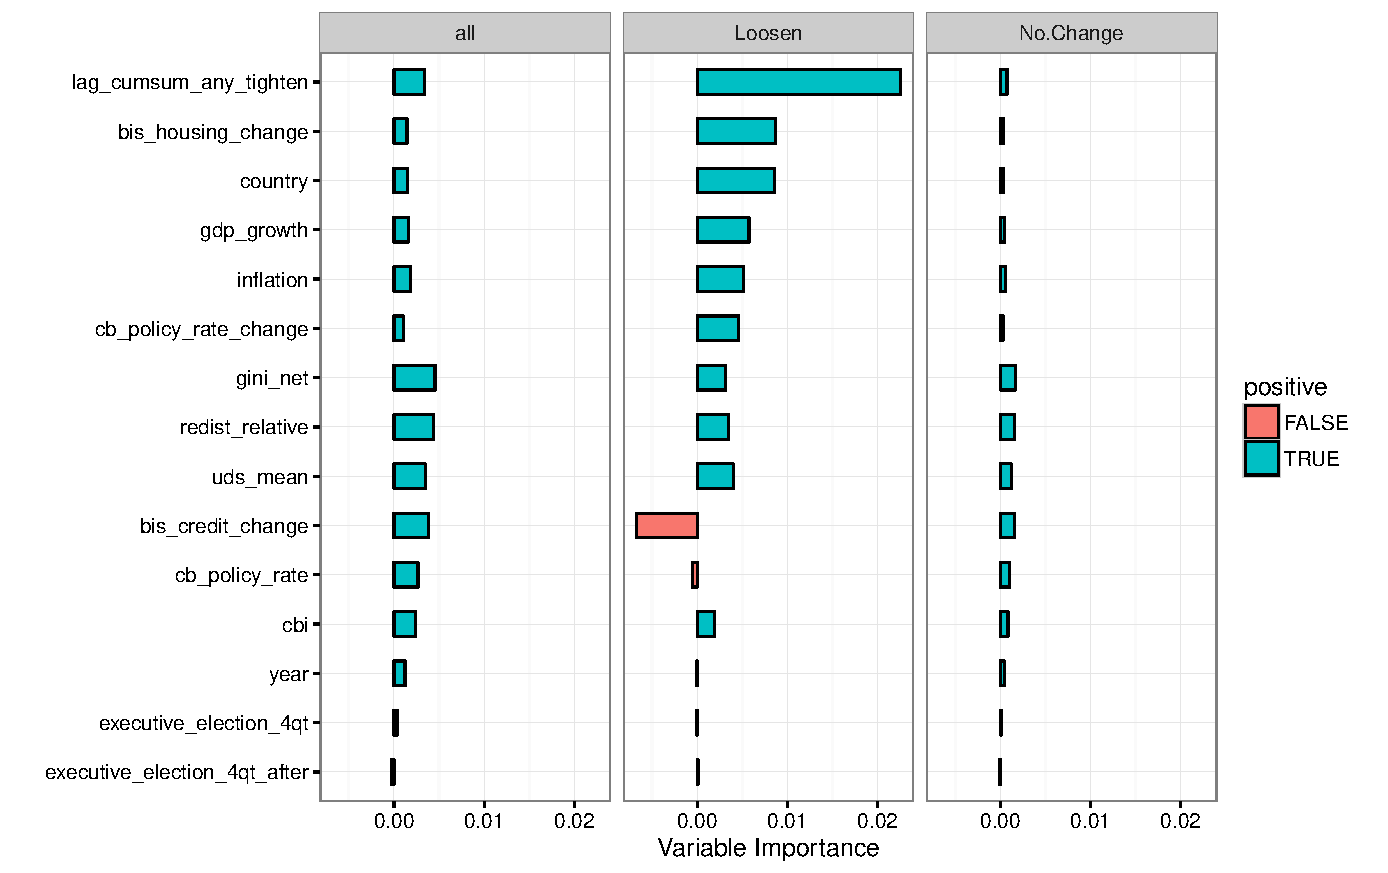
\includegraphics{figures/loosen_imp.pdf}
    \end{center}

    {\scriptsize{Bars coloured by negative or positive variable importance.}}

\end{figure}

\begin{figure}
    \caption{Partial Dependence Plot for Macro-prudential Regulatory Policy Loosening}
    \label{partial_loosen}
    \begin{center}
        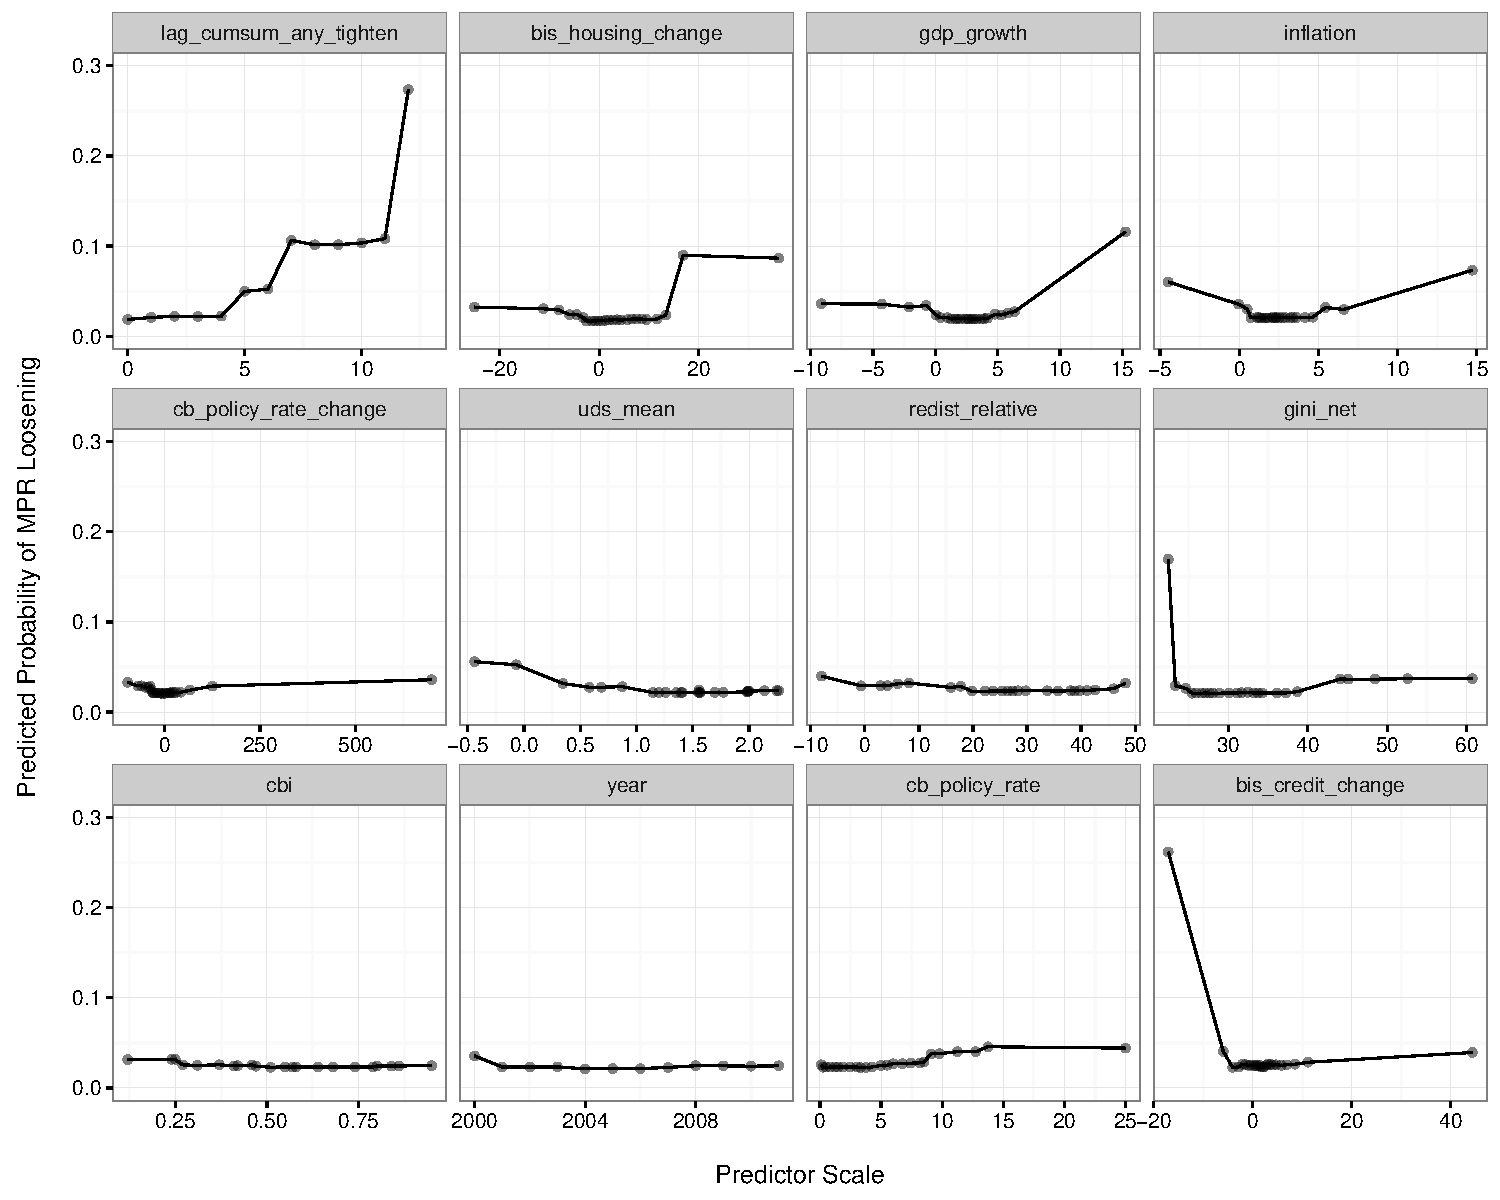
\includegraphics{figures/patial_loosen.pdf}
    \end{center}

    {\scriptsize{Variables shown are those that were below the minimal depth threshold. The "fixed effects" variables are not shown. Note that predictions are for policy change to be made per quarter.}}

\end{figure}

\section{Conclusions}\label{conclusions}

\pagebreak
\renewcommand{\thepage}{A-\arabic{page}}\setcounter{page}{1}
\renewcommand{\thesection}{Appendix \arabic{section}}\setcounter{section}{0}
\renewcommand{\thetable}{A-\arabic{table}}\setcounter{table}{0}
\renewcommand{\thefigure}{A-\arabic{figure}}\setcounter{figure}{0}
\clearpage

\section{Online Appendix}\label{online-appendix}

\subsection{Additional descriptive statistics for the estimation
sample}\label{additional-descriptive-statistics-for-the-estimation-sample}

% latex table generated in R 3.2.4 by xtable 1.8-2 package
% Fri Mar 25 14:35:33 2016
\begin{table}[ht]
\centering
\caption{Country Quarter-Year Sample Included in the Random Forests After Deleting Cases with Missing Values} 
\begingroup\tiny
\begin{tabular}{rlrr}
  \hline
 & Country & First Year & Last Year \\ 
  \hline
1 & Australia & 2004 & 2010 \\ 
  2 & Brazil & 2002 & 2010 \\ 
  3 & Canada & 2000 & 2010 \\ 
  4 & Denmark & 2003 & 2010 \\ 
  5 & Indonesia & 2003 & 2010 \\ 
  6 & Israel & 2000 & 2010 \\ 
  7 & Malaysia & 2005 & 2010 \\ 
  8 & Mexico & 2009 & 2010 \\ 
  9 & New Zealand & 2000 & 2010 \\ 
  10 & Norway & 2000 & 2010 \\ 
  11 & Singapore & 2000 & 2010 \\ 
  12 & South Africa & 2000 & 2010 \\ 
  13 & Sweden & 2003 & 2010 \\ 
  14 & Switzerland & 2000 & 2010 \\ 
  15 & Thailand & 2009 & 2010 \\ 
  16 & United Kingdom & 2000 & 2010 \\ 
  17 & United States & 2000 & 2010 \\ 
   \hline
\end{tabular}
\endgroup
\end{table}


% latex table generated in R 3.2.4 by xtable 1.8-2 package
% Tue Apr 19 10:29:14 2016
\begin{table}[ht]
\centering
\caption{Number of Events and Total Observations for the Random Forests Estimation Sample} 
\label{sampsize}
\begin{tabular}{rrr}
  \hline
Tighten & Loosen & Total \\ 
  \hline
 60 &  24 & 1025 \\ 
   \hline
\end{tabular}
\end{table}


\begin{landscape}
    % latex table generated in R 3.2.4 by xtable 1.8-2 package
% Tue Mar 22 16:18:41 2016
\begin{table}[ht]
\centering
\begingroup\tiny
\begin{tabular}{rrrrrrrrrrr}
  \hline
 & Cum. Tight. (lag) & GDP Growth & GDP/Capita & Inflation & FinStress & Housing Chng & CBI & Election Period & Gini Diff. & UDS \\ 
  \hline
Cum. Tight. (lag) & 1.00 & -0.19 & -0.36 & 0.19 & 0.09 & -0.12 & 0.17 & 0.20 & -0.12 & -0.21 \\ 
  GDP Growth & -0.19 & 1.00 & -0.08 & 0.07 & -0.35 & 0.61 & -0.10 & 0.05 & -0.29 & -0.28 \\ 
  GDP/Capita & -0.36 & -0.08 & 1.00 & -0.43 & 0.02 & 0.04 & -0.38 & -0.20 & 0.48 & 0.51 \\ 
  Inflation & 0.19 & 0.07 & -0.43 & 1.00 & -0.20 & -0.08 & 0.12 & 0.05 & -0.26 & -0.28 \\ 
  FinStress & 0.09 & -0.35 & 0.02 & -0.20 & 1.00 & -0.32 & 0.10 & 0.01 & 0.06 & -0.09 \\ 
  Housing Chng & -0.12 & 0.61 & 0.04 & -0.08 & -0.32 & 1.00 & -0.14 & -0.06 & 0.01 & 0.03 \\ 
  CBI & 0.17 & -0.10 & -0.38 & 0.12 & 0.10 & -0.14 & 1.00 & 0.12 & 0.00 & 0.09 \\ 
  Election Period & 0.20 & 0.05 & -0.20 & 0.05 & 0.01 & -0.06 & 0.12 & 1.00 & -0.12 & -0.12 \\ 
  Gini Diff. & -0.12 & -0.29 & 0.48 & -0.26 & 0.06 & 0.01 & 0.00 & -0.12 & 1.00 & 0.77 \\ 
  UDS & -0.21 & -0.28 & 0.51 & -0.28 & -0.09 & 0.03 & 0.09 & -0.12 & 0.77 & 1.00 \\ 
   \hline
\end{tabular}
\endgroup
\end{table}

\end{landscape}

\subsection{Minimal depth for
tightening}\label{minimal-depth-for-tightening}

Figures \ref{depth_tighten} and \ref{depth_loosen} show the minimal
depths for each variable included in our two random forest models. The
assumption behind these plots is that variables have a higher impact on
predicting MPR policy tightening if they more frequently split nodes
closest to the ``trunk'' of the tree, i.e.~the root node (Ehrlinger
2015b, 11). So a lower minimal depth indicates that the variable is more
important for predicting the MPR policy choice. Using the rule developed
by Ishwaran et al. (2010), minimum depth values below the mean minimum
depth across the variables indicate variables that are important for
predicting MPR choices.\footnote{We used the \texttt{ggRandomForests}
  package (Ehrlinger 2015a) for R to find minimum depths and create
  partial dependence plots shown below.}

\begin{figure}
    \caption{Minimal Depth For Trees Classifying Macro-prudential Policy Tightening}
    \label{depth_tighten}
    \begin{center}
        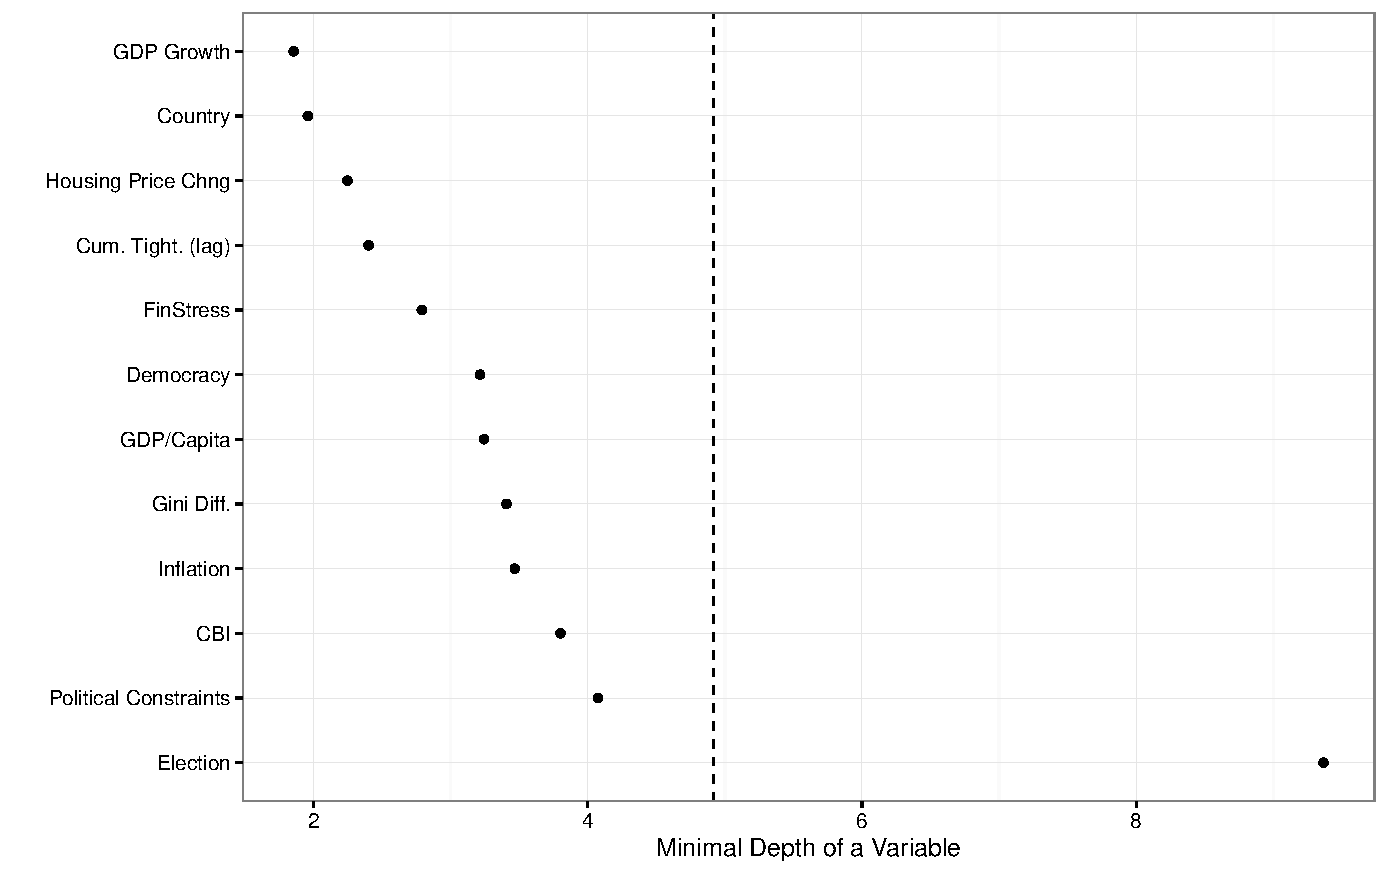
\includegraphics{figures/tighten_md.pdf}
    \end{center}

    {\scriptsize{The dashed vertical line indicates mean minimum depth across the variables. Minimum depths below the mean depth are considered to be important in forest prediction.}}

\end{figure}

\begin{figure}
    \caption{Minimal Depth For Trees Classifying Macro-prudential Policy Loosening}
    \label{depth_loosen}
    \begin{center}
        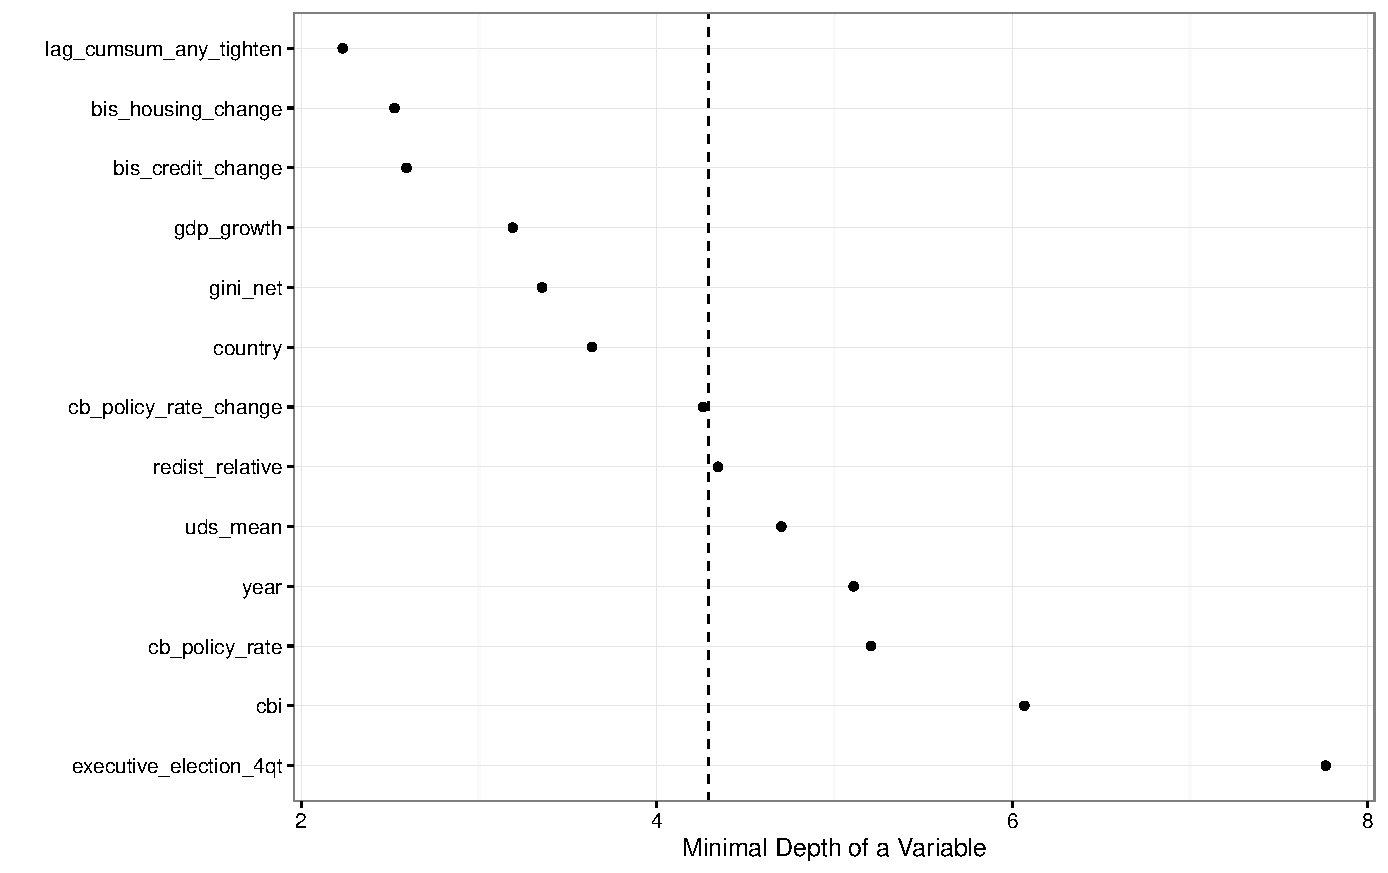
\includegraphics{figures/loosen_md.pdf}
    \end{center}

    {\scriptsize{The dashed vertical line indicates mean minimum depth across the variables. Minimum depths below the mean depth are considered to be important in forest prediction.}}

\end{figure}

\clearpage

\section*{References}\label{references}
\addcontentsline{toc}{section}{References}

\hypertarget{refs}{}
\hypertarget{ref-bis2016}{}
Bank of International Settlements. 2016. ``Residential Property Prices
Selected Series.''

\hypertarget{ref-DPI2001}{}
Beck, Thorsten, George Clarke, Alberto Groff, Philip Keefer, and and
Patrick Walsh. 2001. ``New Tools in Comparative Political Economy: The
Database of Political Institutions.'' \emph{World Bank Economic Review},
no. 1, 15.

\hypertarget{ref-Bodea2015}{}
Bodea, Cristina, and Raymond Hicks. 2015. ``International Finance and
Central Bank Independence: Institutional Diffusion and the Flow and Cost
of Capital.'' \emph{The Journal of Politics} 77 (1): 268--84.

\hypertarget{ref-Breiman1996}{}
Breiman, Leo. 1996. ``Bagging Predictors.'' \emph{Machine Learning} 24
(2): 123--40.

\hypertarget{ref-Breiman2001}{}
---------. 2001. ``Random Forests.'' \emph{Machine Learning} 45 (1):
5--32.

\hypertarget{ref-calomirisHaber2014}{}
Calomiris, Charles W., and Stephen H. Haber. 2014. \emph{Fragile by
Design: The Political Origins of Banking Crises and Scarce Credit}.
Princeton, NJ: Princeton University Press.

\hypertarget{ref-Cukierman1992}{}
Cukierman, Alex, Steven B. Web, and Bilin Neyapti. 1992. ``Measuring the
Independence of Central Banks and Its Effect on Policy Outcomes.''
\emph{The World Bank Economic Review} 6 (3): 353--98.

\hypertarget{ref-r-ggRandomForests}{}
Ehrlinger, John. 2015a. \emph{GgRandomForests: Visually Exploring Random
Forests}. \url{http://cran.r-project.org/package=ggRandomForests}.

\hypertarget{ref-Ehrlinger2015}{}
---------. 2015b. ``ggRandomForests.'' \emph{Arxiv Working Paper},
February, 1--30.

\hypertarget{ref-ilzetzki2010}{}
Ethan Ilzetzki, Carmen M. Reinhart, and Kenneth S. Rogoff. 2010.
``Exchange Rate Arrangements Entering the 21st Century: Which Anchor
Will Hold?''

\hypertarget{ref-Friedman2000}{}
Friedman, JH. 2000. ``Greedy Function Approximation: A Gradient Boosting
Machine.'' \emph{Annals of Statistics} 20: 1189--1232.

\hypertarget{ref-GandrudHallbergFinStress}{}
Gandrud, Christopher, and Mark Hallerberg. 2015. ``What Is a Financial
Crisis? Efficiently Measuring Real-Time Perceptions of Financial Market
Stress with an Application to Financial Crisis Budget Cycles.''
\emph{CESIfo Working Paper}, no. 5632.

\hypertarget{ref-Gelman2008}{}
Gelman, Andrew, Aleks Jakulin, Maria Grazia Pittau, and Yu-Sung Su.
2008. ``A weakly informative default prior distribution for logistic and
other regression models.'' \emph{The Annals of Applied Statistics} 2
(4): 1360--83.

\hypertarget{ref-hill2014empirical}{}
Hill, Daniel W, and Zachary M Jones. 2014. ``An Empirical Evaluation of
Explanations for State Repression.'' \emph{American Political Science
Review} 108 (03). Cambridge Univ Press: 661--87.

\hypertarget{ref-hyde2012}{}
Hyde, Susan D., and Nikolay Marinov. 2012. ``Which Elections Can Be
Lost?'' \emph{Political Analysis} 20 (2): 191--201.

\hypertarget{ref-imfifs}{}
International Monetary Funds. 2016. ``International Financial
Statistics.''

\hypertarget{ref-Ishwaran2010}{}
Ishwaran, H, UB Kogalur, EZ Gorodeski, AJ Minn, and MS Lauer. 2010.
``High-Demensional Variable Selection for Survival Data.'' \emph{Journal
of the American Statistical Association} 105: 205--7.

\hypertarget{ref-jones2015}{}
Jones, Zachary, and Fridolin Linder. 2015. ``Exploratory Data Analysis
Using Random Forests.'' \emph{Paper Presented at the Annual MPSA
Conference}.

\hypertarget{ref-king2001logistic}{}
King, Gary, and Langche Zeng. 2001. ``Logistic Regression in Rare Events
Data.'' \emph{Political Analysis} 9 (2): 137--63.

\hypertarget{ref-lim2013}{}
Lim, Cheng Hoon, Ivo Krznar, Fabian Lipinsky, Akira Otani, and Xiaoyong
Wu. 2013. ``The Macroprudential Framework: Policy Responsiveness and
Institutional Arrangements.'' \emph{IMF Working Paper} WP/13/166.

\hypertarget{ref-Muchlinski2016}{}
Muchlinski, David, David Siroky, Jingrui He, and Matthew Kocher. 2016.
``Comparing Random Forest with Logistic Regression for Predicting
Class-Imbalanced Civil War Onset Data.'' \emph{Political Analysis} 24
(1): 87--103.

\hypertarget{ref-Pemstein2010}{}
Pemstein, Daniel, Stephen A. Meserve, and James Melton. 2010.
``Democratic Compromise: A Latent Variable Analysis of Ten Measures of
Regime Type.'' \emph{Political Analysis} 18 (4): 426--49.

\hypertarget{ref-piketty2013top}{}
Piketty, Thomas, and Emmanuel Saez. 2013. ``Top Incomes and the Great
Recession: Recent Evolutions and Policy Implications.'' \emph{IMF
Economic Review} 61 (3). Nature Publishing Group: 456--78.

\hypertarget{ref-rajan2012fault}{}
Rajan, Raghuram. 2012. \emph{Fault Lines: How Hidden Fractures Still
Threaten the World Economy}. Princeton, NJ: Princeton University Press.

\hypertarget{ref-dReinhardt2015}{}
Reinhardt, Dennis, and Rhiannon Sowerbutts. 2015. ``Regulatory arbitrage
in action: evidence from banking flows and macroprudential policy.''
\emph{Bank of England Staff Working Paper}, September, 1--37.

\hypertarget{ref-bis2014}{}
Scatigna, Michela, Robert Szemere, and Kostas Tsatsaronis. 2014.
``Residential Propoerty Price Statistics Across the Globe.'' \emph{BIS
Quarterly Reivew} September.

\hypertarget{ref-shellman2013shifting}{}
Shellman, Stephen M, Brian P Levey, and Joseph K Young. 2013. ``Shifting
Sands Explaining and Predicting Phase Shifts by Dissident
Organizations.'' \emph{Journal of Peace Research} 50 (3). SAGE
Publications: 319--36.

\hypertarget{ref-solt2008economic}{}
Solt, Frederick. 2008. ``Economic Inequality and Democratic Political
Engagement.'' \emph{American Journal of Political Science} 52 (1). Wiley
Online Library: 48--60.

\hypertarget{ref-Solt2014}{}
---------. 2014. ``The Standardized World Income Inequality Database.''
\emph{Working Paper}.

\hypertarget{ref-spirling2012us}{}
Spirling, Arthur. 2012. ``US Treaty Making with American Indians:
Institutional Change and Relative Power, 1784--1911.'' \emph{American
Journal of Political Science} 56 (1). Wiley Online Library: 84--97.

\hypertarget{ref-worldbank2016}{}
World Bank. 2016. ``The Global Financial Development Database.''

\end{document}
